\documentclass[../document.tex]{subfiles}
%\documentclass{beamer}
\usepackage{amssymb,amsmath,amsthm}
\usepackage{graphicx}
\usepackage{tikz}
%\usetheme{Singapore}
\usetheme{Boadilla}
\usecolortheme{rose}

\usetikzlibrary{tikzmark}
\usepackage{colortbl}
\usepackage{graphicx}
\usepackage{pdfpages}
\tikzstyle{every picture}+=[remember picture,baseline]
\tikzstyle{every node}+=[inner sep=0pt,anchor=base,
minimum width=1.5cm,align=center,text depth=.25ex,outer sep=1.5pt]
\tikzstyle{every path}+=[thick, rounded corners]
%\setframetemplate{frametitle}[default][center]

%%%%%%%%%%%%%%%%%%%% VERY IMPORTANT 
%very useful way to add notes to Beamer
%\setbeameroption{show notes on second screen=right}
\setbeamertemplate{note page} 
{ 
	\insertslideintonotes{0.65} 
	\rule{\textwidth}{0.1pt} 
	\color{blue} \small
	\insertnote 
}

\begin{document}
	
\begin{frame}
	\frametitle{Brief history of the origination of the problem}
	\begin{itemize}
		\item<1-> \textbf{Naming:} "Because it was posed as a cute problem about philosophers seated around a table, \textbf{Dijkstra’s dining philosopher’s problem} received much more attention than it deserves. (For example, it has probably received more attention in the theory community than the readers/writers problem, which illustrates the same principles and has much more practical importance.) … The popularity of the dining philosophers problem taught me that \textbf{the best way to attract attention to a problem is to present it in terms of a story}." -Lamport
		\item<2-> \textbf{Motivation:} Two General's problem. \uncover<3->{Byzantine General is a rather more general form of this problem.}
	\end{itemize}
\end{frame}

%%%%%%%%%%%

\begin{frame}
	\frametitle{A brief Overview of Two general's problem}
	\framesubtitle {\large Stating the problem through visualization!}
	\begin{tikzpicture}[remember picture,overlay]
		\node[above=1cm] at(current 	page.south) { %for relative positioning, we use \node [left=1cm or right or below or above] 
			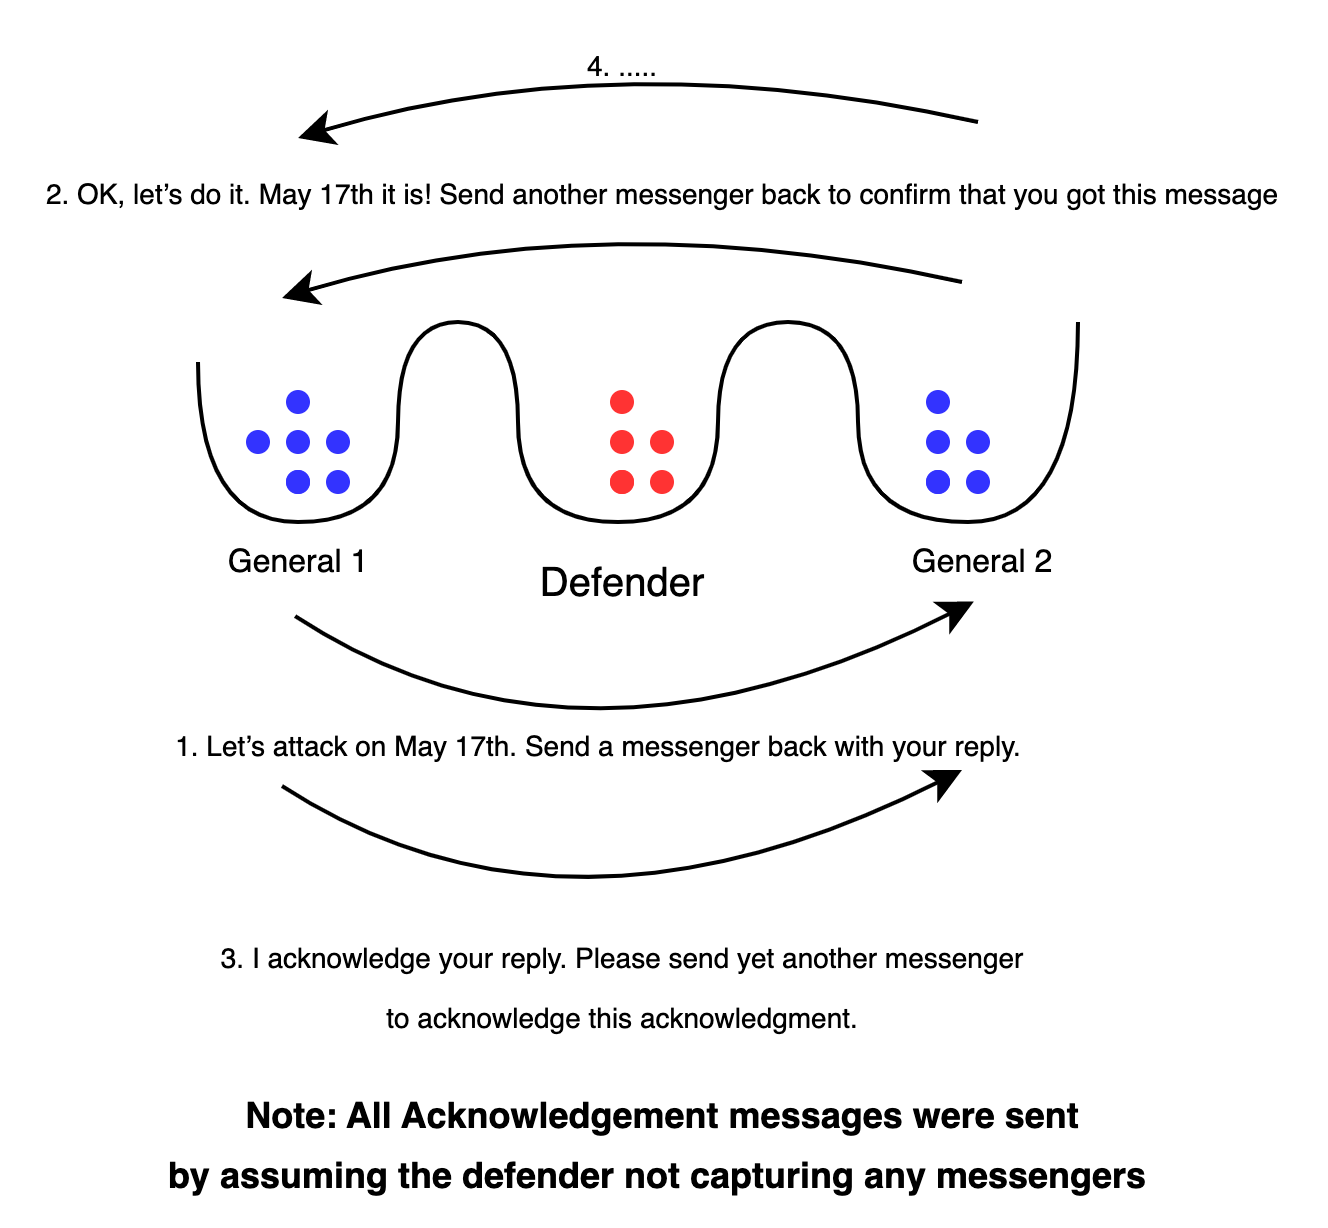
\includegraphics[width=0.6\textwidth]{../myfig2.png}	
		};
	\end{tikzpicture}
\end{frame}
\end{document}